\subsection*{Log ud}
Log ud-funktion kan tilgås fra hovedmenuen og tillader brugeren at logge ud af systemet. Dette medvirker til, at brugeren ikke forbliver logget ind og tillader at andre  kan logge ind på samme app.
Aktiviteterne for log ud fremgår af \autoref{fig:logud}.

\begin{figure} [H]
\centering
\textbf{Aktivitetsdiagram: Log ud}\par\medskip
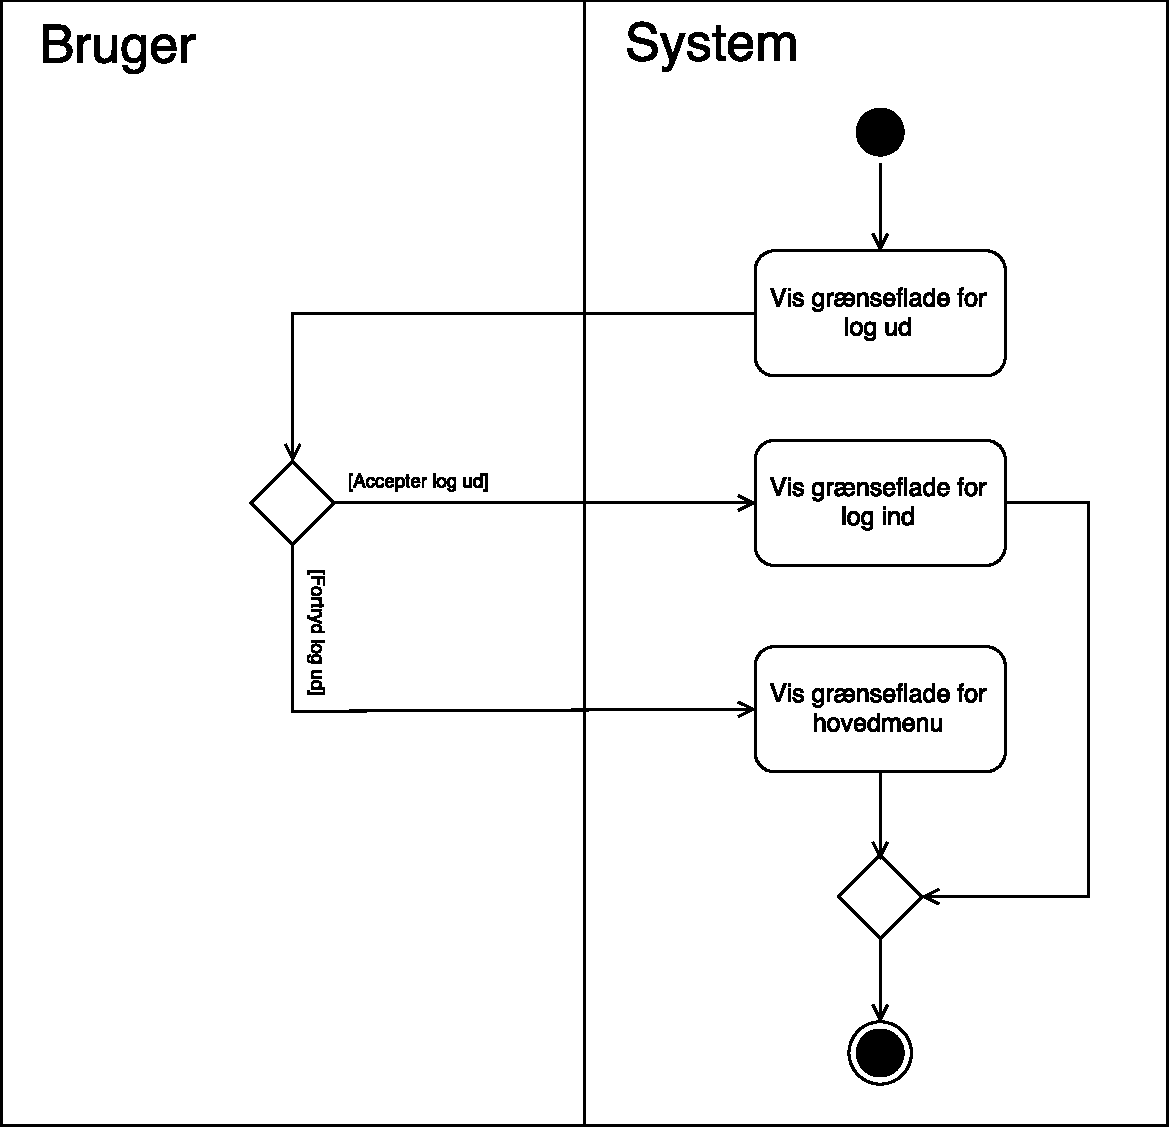
\includegraphics[width=0.9\textwidth]{figures/aktivitetsdiagram/Logud}
\caption{Aktivitetsdiagram over log ud.}
\label{fig:logud}
\end{figure}

\noindent
Vælger brugen at logge ud, vises grænsefladen for log ud. Brugeren skal efterfølgende bekræfte, at de ønsker at logge ud. Ønskes dette, logges brugeren ud og grænsefladen for log ind vises. Fortryder brugeren at logge ud, vil systemet returnere til hovedmenuen og grænsefladen for denne vises. 